\documentclass[Orbiter User Manual.tex]{subfiles}
\begin{document}

\section{The main menu}
\label{sec:menu}
The main menu is displayed at the top centre of the simulation window. It provides access to various functions and control dialogs. To the left and right of the menu bar, additional information panels may be shown.\\
If the menu bar is not visible, move the mouse pointer towards the top edge of the simulation window to scroll it down. Alternatively, pressing \keystroke{F4} will show or hide the menu bar.\\
The behaviour of the menu and info panels can be defined via the menu configuration dialog, which can be accessed by right-clicking on the menu bar.

\begin{figure}[H]
	\centering
	\subfigure{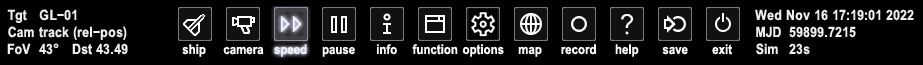
\includegraphics[width=0.99\textwidth]{main_menu.png}}
	\caption{Menu bar and info panels}
\end{figure}

\noindent
\textbf{Menu options:}

\begin{itemize}
\item \textbf{ship:} Open the Vessel selection dialog which allows to switch input focus to a different spacecraft in the simulation (see section \ref{ssec:menu_vessel_sel}). Keyboard shortcut: \keystroke{F3}.
\item \textbf{camera:} Open the Camera dialog which allows to configure the observer camera, including camera target selection, positioning, field of view and track mode (see section \ref{ssec:menu_camera}). Keyboard shortcut: \Ctrl\keystroke{F1}.
\item \textbf{speed:} Open the Simulation speed dialog, which provides access to time acceleration settings, and allows pausing/resuming the simulation (see section \ref{ssec:menu_time}). Keyboard shortcut: \Ctrl\keystroke{F2}.
\item \textbf{pause:} pause/resume the simulation. Keyboard shortcut: \Ctrl\keystroke{P}.
\item \textbf{info:} Open the Object info dialog which displays live information for all simulation objects (see section \ref{ssec:menu_info}). Keyboard shortcut: \Ctrl\keystroke{I}.
\item \textbf{function:} Open the Custom function dialog which lists all accessible functions provided by active external modules, if available (see section \ref{ssec:menu_cust_func}). Keyboard shortcut: \Ctrl\keystroke{F4}.
\item \textbf{options:} Open the Options dialog which allows to configure functional and visual simulation parameters, such as MFD parameters, joystick settings, celestial sphere background rendering settings, or "Visual helpers" (see section \ref{ssec:menu_options}). Keyboard shortcut: \keystroke{F6}.
\item \textbf{map:} Open the Map window for a planetary body, including day/night terminator lines, orbital planes or ground tracks and planetary surface markers (see section \ref{ssec:menu_map}). Keyboard shortcut: \Ctrl\keystroke{M}.
\item \textbf{record:} Open the Record/playback dialog which allows to record a simulation session, or configure the playback parameters during a replay (see section \ref{sec:flight_rec}). Keyboard shortcut: \Ctrl\keystroke{F5}.
\item \textbf{help:} Open the inline Help dialog window (see section \ref{ssec:menu_help}). Keyboard shortcut: \Alt\keystroke{F1}.
\item \textbf{save:} Saves the current simulation state to the Quicksave scenario folder. Keyboard shortcut: \Ctrl\keystroke{S}.
\item \textbf{exit:} Quit the simulation session and return to the Launchpad dialog. Keyboard shortcuts: \Ctrl\keystroke{Q} or \Alt\keystroke{F4}.
\end{itemize}

\noindent
\textbf{Additional info panels:}

\begin{itemize}
\item The panel in the top left corner of the simulation window contains the name of the camera target (Tgt), the camera mode (Cam) and the field of view angle (FoV).
\item The panel in the top right corner contains the date in Ephemeris Time (ET) and in Modified Julian Day (MJD) format, the simulation elapsed time (Sim) in seconds, as well as indicators for pause, time acceleration and record/playback if applicable.

\infobox{Orbiter provides a date conversion utility (date.exe) in the \textit{Utils} subdirectory. The \textit{Scenario Editor} (see section \ref{ssec:scn_editor}) allows to manipulate the date of a running simulation.}

\item Optionally, two more info panels can be displayed by user selection from the menu configuration dialog, including a frame rate display, a render statistics display showing the graphics engine load, or a viewport info display.
\end{itemize}


\subsection{Vessel selection}
\label{ssec:menu_vessel_sel}
The \textit{Vessel selection} dialog can be used to switch to a different spacecraft in the simulation session, if available. It is opened with the \textit{ship} button from the main menu (keyboard shortcut \keystroke{F3}).

\begin{figure}[H]
	\centering
	\subfigure{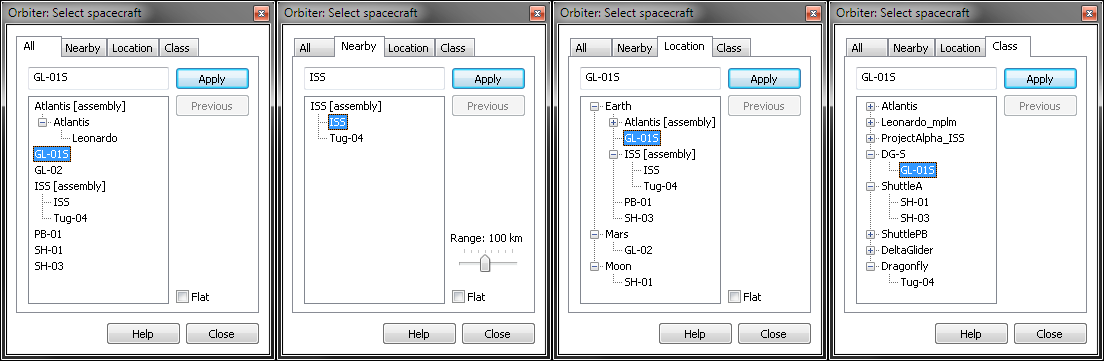
\includegraphics[width=0.99\textwidth]{vessel_sel.png}}
\end{figure}

\noindent
You can pick a vessel from the list and click Apply to jump into a new spacecraft. Clicking Previous puts you back into the original ship. (\Ctrl\keystroke{F3} is a shortcut to switch between the two most recent vessels.)\\
The tab pages (All, Nearby, Location, Class) present the vessel list sorted according to different criteria:

\begin{itemize}
\item \textbf{All:} shows all vessels in the current simulation session.
\item \textbf{Nearby:} shows only vessels in the vicinity of the current focus vessel. The search radius can be adjusted with the slider on the right.
\item \textbf{Location:} Groups the vessels according to the closest celestial body.
\item \textbf{Class:} Groups the vessels according to type (vessel class).
\end{itemize}

\noindent
Vessel assemblies (spacecraft that consist of multiple docked components) are normally represented as groups, listing the component vessels as sub-entries of the assembly. The Flat option shows the vessels in a flat list instead, regardless of their connections.\\
Note that only vessels which accept user input focus appear in the list. Vessels and components which don't support individual manual control, such as the Space Shuttle's booster rockets (SRBs) or external tank which are managed from the Shuttle orbiter, are omitted.


\subsection{Camera control}
\label{ssec:menu_camera}
The \textit{Camera} dialog offers various ways to select viewpoints, camera targets or movement modes. It can be accessed via the \textit{camera} button on the main menu (keyboard shortcut \Ctrl\keystroke{F1}).\\
\\
\textbf{Control tab:}\\
This tab contains controls for moving and tilting the viewer camera. The available options depend on the current camera mode.

\begin{figure}[H]
	\centering
	\subfigure{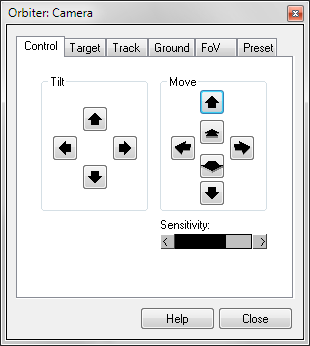
\includegraphics[width=0.35\textwidth]{tab_control.png}}
\end{figure}

\noindent
In internal (cockpit) views, the camera can be rotated to allow the pilot to look around (keyboard shortcuts \Alt\DArrow\UArrow\RArrow\LArrow$_{Cur}$, or alternatively right-click and drag the mouse). The view direction can be re-centred with the Forward button (shortcut \Home$_{Cur}$).\\
In external views the camera can be rotated around the target (keyboard shortcuts \Ctrl\DArrow\UArrow\RArrow\LArrow$_{Cur}$ or right-click and drag the mouse). It can also be moved towards or away from the target (shortcuts \keystroke{PageUp}\keystroke{PageDown}$_{Cur}$ or mouse wheel).\\
In ground-based views, the camera can be tilted (shortcuts \DArrow\UArrow\RArrow\LArrow$_{Cur}$), panned (shortcuts \Ctrl\DArrow\UArrow\RArrow\LArrow$_{Cur}$) or raised and lowered (shortcuts \keystroke{PageUp}\keystroke{PageDown}$_{Cur}$) unless locked onto a target, in which case it can only be rotated around the target (shortcuts \Ctrl\RArrow\LArrow$_{Cur}$), moved towards or away from the target (shortcuts \Ctrl\DArrow\UArrow$_{Cur}$). Raising and lowering the camera is also possible in target-locked mode.\\
The Sensitivity slider can be used to adjust the speed of movement.\\
\\
\textbf{Target tab:}\\
This tab provides a list of potential camera targets (vessels, celestial bodies, spaceports). Click on an object in the list and Apply to set a new camera target. Note that setting a new vessel target does not automatically switch the input focus. To do that, use the \textit{Vessel selection} dialog (see section \ref{ssec:menu_vessel_sel}). You can switch the camera back to the vessel you are controlling by pressing the Focus cockpit or Focus extern buttons (shortcut \keystroke{F1}).\\

\begin{figure}[H]
	\centering
	\subfigure{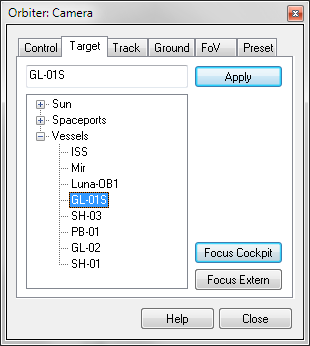
\includegraphics[width=0.35\textwidth]{tab_target.png}}
\end{figure}

\noindent
Note that after selecting a new camera target, you may need to adjust the distance (\keystroke{PageUp}\keystroke{PageDown}$_{Num}$).\\
\\
\textbf{Track tab:}\\
Allows to select different camera track modes which determine how the camera moves around and follows the target.\\

\begin{figure}[H]
	\centering
	\subfigure{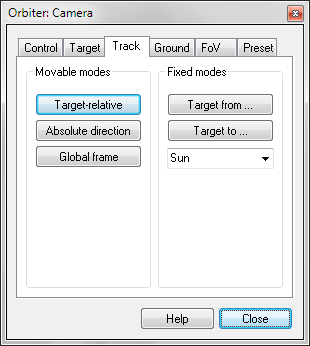
\includegraphics[width=0.35\textwidth]{tab_track.png}}
\end{figure}

\noindent

\begin{itemize}
\item \textbf{Target-relative:} camera maintains its position and orientation relative to the target. Camera movement is aligned with the vessel axes.
\item \textbf{Absolute direction:} Movement is still aligned with the vessel axes, but the camera keeps looking in a fixed direction even if the target is rotating.
\item \textbf{Global frame:} The camera still follows the target, but maintains a fixed orientation in a global frame of reference.
\item \textbf{Target from:} This mode places the camera so that the observer looks at the target from the direction of a specified reference object. For example, Target from Sun always places the Sun behind the observer, so always shows the lit side of the target. Unlike the first three track modes, this mode fixes the camera position and doesn't allow rotation around the target.
\item \textbf{Target to:} Similar to Target from, but this mode places the reference object behind the target. So for example, Target to Sun makes the camera look into the Sun, and shows the unlit side of the target.
\end{itemize}

\noindent
A keyboard shortcut for cycling between the first three track modes is \keystroke{F2}.\\
\\
\textbf{Ground tab:}\\
This page allows setting the camera into a surface-relative position and orientation. Unlike the track modes, the camera doesn't follow the target, but stays fixed relative to the planet surface. It can be set up either in \textit{free} mode, or in \textit{target lock} mode, where it keeps looking in the direction of the target. Use the Target lock check box to choose between the two modes.

\begin{figure}[H]
	\centering
	\subfigure{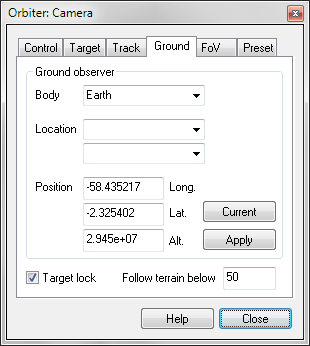
\includegraphics[width=0.35\textwidth]{tab_ground.png}}
\end{figure}

\noindent
You can either manually set the surface location (latitude/longitude) and altitude on a reference planet and press Apply, or just press Current to put the camera into ground mode at its current location relative to the reference planet.

\infobox{When the camera is in free ground mode, it is no longer linked to a target object, so picking targets in the \textit{Target} tab will not have an effect in this mode, but the new target will be used when switching back to a target-tracking mode.}

\noindent
\textbf{FoV tab:}\\
This page allows adjustment of the camera field of view (FoV), i.e. the camera zoom setting. The FoV can be set in discrete steps by clicking the buttons (30°-70°) or continuously by moving the slider, in the range 10°-90°. The FoV is measured between the top and bottom edges of the view window.

\begin{figure}[H]
	\centering
	\subfigure{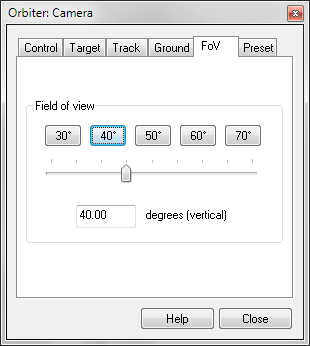
\includegraphics[width=0.35\textwidth]{tab_fov.png}}
\end{figure}

\noindent
Keyboard shortcuts: \keystroke{Z}/\keystroke{X} for continuous FoV adjustment, or \Ctrl+\keystroke{Z}/\keystroke{X} for discrete adjustments in steps of 10°.

\infobox{Separate FoV settings are used for internal (cockpit) and external views, and adjusting one will not affect the other. Jumping between internal and external views will switch the FoV values to their respective settings.}

\noindent
\textbf{Preset tab:}\\
Orbiter provides an easy method to store and recall camera modes in a preset list. Click on the \textit{Preset} tab in the camera dialog. Any available modes are listed here. To activate a mode, double-click it in the list, or select the mode and click Recall.

\begin{figure}[H]
	\centering
	\subfigure{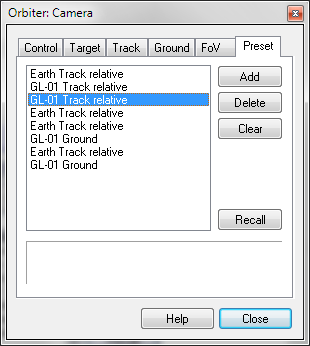
\includegraphics[width=0.35\textwidth]{tab_preset.png}}
\end{figure}

\noindent
To store the current camera mode as a new preset in the list, simply click Add. This will produce a new entry with a short description. To delete a mode, click Delete, or Clear to clear the whole list.\\
Each entry remembers its track mode, position, target and FoV. The preset list is a good way to prepare a set of camera angles beforehand (for example to follow a launch) and then activate them quickly without having to adjust the positions manually. The preset list is stored together with the simulation state, so it can be shared via a scenario file.


\subsection{Time acceleration}
\label{ssec:menu_time}
Spaceflight missions can take take weeks, months or even years in real time. If you plan a trip to the outer planets, running the simulation in real time is impractical, so Orbiter provides a time acceleration feature to fast-forward through coasting phases where nothing much is happening.

\begin{figure}[H]
	\centering
	\subfigure{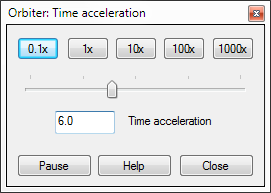
\includegraphics[width=0.35\textwidth]{time_accel.png}}
\end{figure}

\noindent
Open the \textit{Time acceleration} dialog with the speed button on the main menu (keyboard shortcut: \Ctrl\keystroke{F2}). Time can be accelerated up to 1000x in discrete steps with the buttons, or continuously with the slider. It can also be slowed town to one tenth of real time. Keyboard shortcuts are \keystroke{T} for speeding up by a factor of 10, and \keystroke{R} for slowing down by a factor of 10. The maximum time acceleration supported with the keyboard shortcuts is 100000x, compressing a year into approximately 5 minutes.
\\
\alertbox{High time accelerations can affect the accuracy and stability of the simulation, in particular close to planetary bodies or in the atmosphere, because the intervals between time frames become too large to allow precise integration of the vessel state vectors. Use high time accelerations only far from gravitational sources in interplanetary space.
Always switch back to real time before firing thrusters or other manual control actions. Things happen too fast even at moderate time accelerations to make it practical during manual manoeuvres.}
\noindent
\\
The dialog also provides a button for pausing/resuming the simulation (shortcut: \Ctrl\keystroke{P}). This function is also directly available from the main menu.


\subsection{Object info}
\label{ssec:menu_info}
The \textit{Object info} window displays data about spacecraft, celestial bodies and spaceports. It can be opened with the \textit{info} button on the main menu (keyboard shortcut \Ctrl\keystroke{I}).\\
After opening, the window shows data for the focus vessel currently controlled by the user. Different objects can be selected from the drop-down lists at the top of the window. The information presented depends on the object type. Data are grouped into categories. Categories can be expanded or collapsed individually, or collectively with the controls at the bottom of the window.\\
The Map button opens the \textit{Map} window (see section \ref{ssec:menu_map}) automatically focussed on the selected target.\\
\\
\textbf{Vessel info}\\
For vessel objects, the info panel shows information categories

\begin{figure}[H]
	\centering
	\subfigure{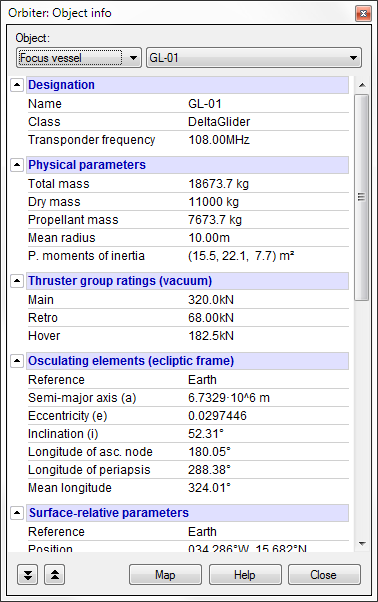
\includegraphics[width=0.4\textwidth]{info_vessel.png}}
\end{figure}

\noindent
\begin{itemize}
\item \textbf{Designation:} vessel name and class, transponder frequency
\item \textbf{Physical parameters:} mass (total, dry, propellant), size and inertia moments
\item \textbf{Thruster ratings:} vacuum thrust for main, retro and hover thruster groups
\item \textbf{Osculating elements:} current 2-body orbital elements with respect to the reference body in the ecliptic frame (semi-major axis, eccentricity, inclination, longitude of ascending node, longitude of periapsis, mean longitude at epoch)
\item \textbf{Surface-relative parameters:} position, velocity and orientation relative to the closest planetary body (longitude/latitude, altitude, ground speed, vertical speed, heading, pitch and bank angles)
\item \textbf{Aerodynamic parameters:} the vessel's current dynamic pressure, true airspeed, Mach number, lift, drag and weight forces, lift/drag ratio, and angle of attack
\item \textbf{Docking ports:} status (free/docked vessel designation), IDS frequency (if applicable) for each of the vessel's docking ports
\item \textbf{State propagation:} update mode (active/idle). For active vessels, shows current state vector propagation integrator, intra-frame subsamples and the gravity sources currently included in the computation
\end{itemize}

\noindent
\\
\textbf{Spaceport info}\\
For surface-based spaceports, the info panel shows categories

\begin{figure}[H]
	\centering
	\subfigure{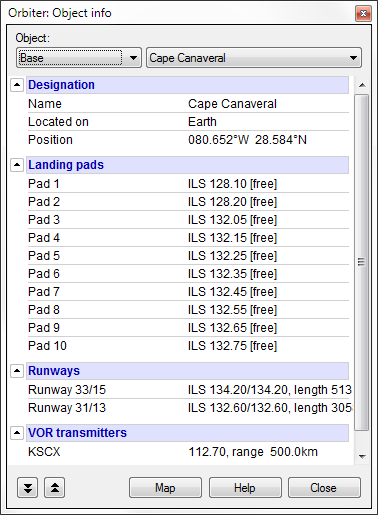
\includegraphics[width=0.4\textwidth]{info_base.png}}
\end{figure}

\noindent
\begin{itemize}
\item \textbf{Designation:} base name, planet and position (longitude/latitude)
\item \textbf{Landing pads:} Lists all VTOL pads available at the base, with status (free/landed vessel designation) and ILS frequency (if available)
\item \textbf{Runways:} List all available runways, with 2-digit designation (including reverse direction, ILS frequencies (if available) and runway lengths
\item \textbf{VOR transmitters:} omni-directional position beacons located directly at the base (if available)
\end{itemize}

\noindent
For a more complete picture of the VOR stations located around the base, open the \textit{Map} window, enable VOR stations in the options, and zoom into the target base until VOR frequencies are shown.\\
\\
\textbf{Celestial body info}\\
For celestial bodies (sun, planets, moons, minor bodies), the info window shows categories

\begin{figure}[H]
	\centering
	\subfigure{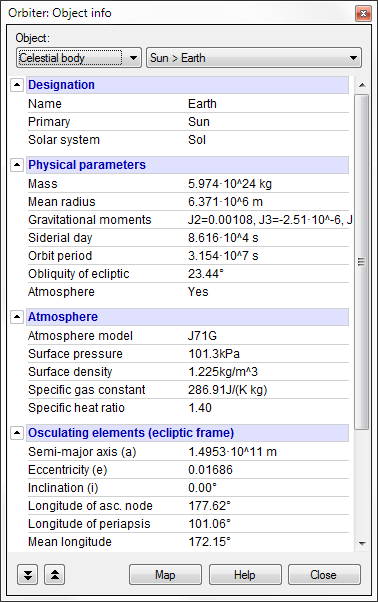
\includegraphics[width=0.4\textwidth]{info_celestial.png}}
\end{figure}

\noindent
\begin{itemize}
\item \textbf{Designation:} name, primary (parent) body and solar system designation
\item \textbf{Physical parameters:} mass, mean radius, parameters of the gravitational moments (J$_{X}$), if available, sidereal day length, orbital period, obliquity (axis tilt against ecliptic plane), atmosphere model active
\item \textbf{Atmosphere (if modelled):} model name, surface pressure and density, specific gas constant, specific heat ratio
\item \textbf{Osculating elements:} current 2-body orbital elements with respect to the parent body in the ecliptic frame (semi-major axis, eccentricity, inclination, longitude of ascending node, longitude of periapsis, mean longitude at epoch)
\item \textbf{Ecliptic position from primary:} longitude, latitude in the ecliptic frame, distance from primary
\item \textbf{State propagation:} analytic (from module): state vectors at arbitrary times available from dedicated module, or dynamic: via sequential state vector propagation
\end{itemize}


\subsection{Map}
\label{ssec:menu_map}
The \textit{Map} window shows a planetary surface represented by coastlines and contours in cylindrical projection. It contains the locations of surface bases and navigation radio transmitters, as well as the location and ground track of orbiting objects. The Map window is opened with the map button in the main menu (shortcut: \Ctrl\keystroke{M}).

\begin{figure}[H]
	\centering
	\subfigure{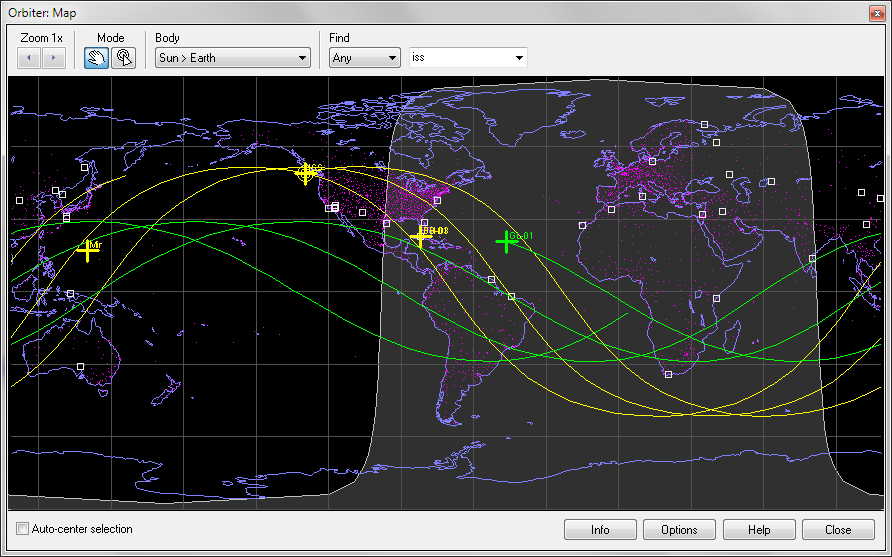
\includegraphics[width=0.99\textwidth]{map.png}}
\end{figure}

\noindent
\textbf{Controls:}

\begin{itemize}
\item \textbf{Zoom:} Use the buttons to zoom in and out of the map. You can also resize the map window to get a more detailed view.
\item \textbf{Mode:} Switch between click and drag (only available if auto-center is disabled) and object selection modes.
\item \textbf{Body:} Change the map to a different planetary body. The list is hierarchical. It lists the current body, its children and parent. To select a sibling body (e.g. go from one planet to another) you first have to pick their parent (e.g. the sun).
\item \textbf{Find:} Select an object by type and name. Typing the first few characters opens a drop-down list to pick from.
\item \textbf{Auto-center selection:} Keep the map centred on the currently selected object.
\item \textbf{Info:} Open the Object info window for the currently selected object (see section \ref{ssec:menu_info}).
\item \textbf{Options:} Open the map configuration dialog.
\end{itemize}

\noindent
\\
\textbf{Configuration:}

\begin{figure}[H]
	\centering
	\subfigure{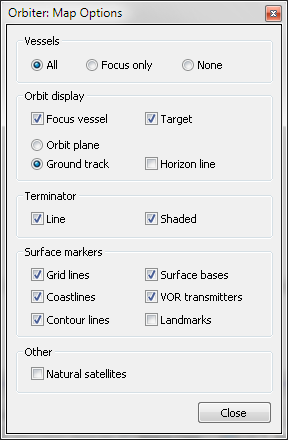
\includegraphics[width=0.35\textwidth]{map_options.png}}
\end{figure}

\begin{itemize}
\item \textbf{Vessels:} \textit{All} (show all spacecraft currently landed on/orbiting this celestial body), \textit{Focus only} (show only the user-controlled vessel, if it is landed on or orbiting the body), \textit{None} (disable vessel objects)
\item \textbf{Orbit display:} show orbit representations for the current focus vessel (the user-controlled vessel) and/or target vessel (the vessel selected in the map, if any). The map can display either the orbit plane (the intersection of the current orbital plane with the celestial body surface) for these orbits, or the predicted ground track for the next few orbits (assuming that the orbital elements don't change). The horizon line for those vessels can also be displayed (the extent of the planet surface visible from the current vessel position and altitude).
\item \textbf{Surface markers:} Show or hide various types of terrain data and surface objects: Grid lines (30° latitude/longitude lines), coastlines (if applicable), contour lines (if available), surface bases (the registered spaceports located on the planet), VOR transmitters (omnidirectional navigation beacons), and landmarks.
\item \textbf{Other:} Natural satellites: show or hide the location above the surface of any moons orbiting the planet.
\end{itemize}


\subsection{Options}
\label{ssec:menu_options}
In addition to global simulation parameters which must be defined before launching an Orbiter session (see Launchpad dialog, section \ref{sec:launchpad}), some aspects of the simulation can be configured during a running simulation from the \textit{Options} dialog, which can be accessed via the \textit{options} button on the main menu (keyboard shortcut: \keystroke{F6}).

\begin{figure}[H]
	\centering
	\subfigure{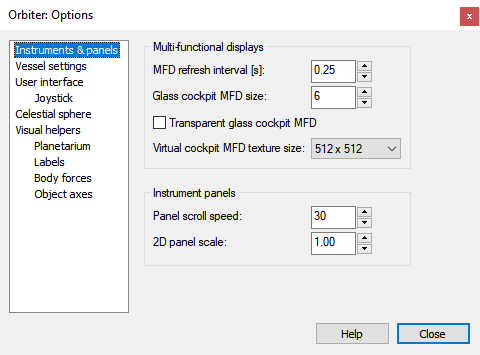
\includegraphics[width=0.5\textwidth]{options.png}}
\end{figure}

\noindent
The "Visual helpers" page can be accessed directly via keys \Ctrl\keystroke{F9}.\\
The parameters in these option pages are explained in the Launchpad Options subsection (see section \ref{ssec:options_tab}).


\subsection{Inline help}
\label{ssec:menu_help}
The help button on the main menu (shortcut: \Ctrl\keystroke{F1}) opens the inline help window accessible during a simulation session. The help window can also be called up from the Orbiter Launchpad by clicking the Help button.

\begin{figure}[H]
	\centering
	\subfigure{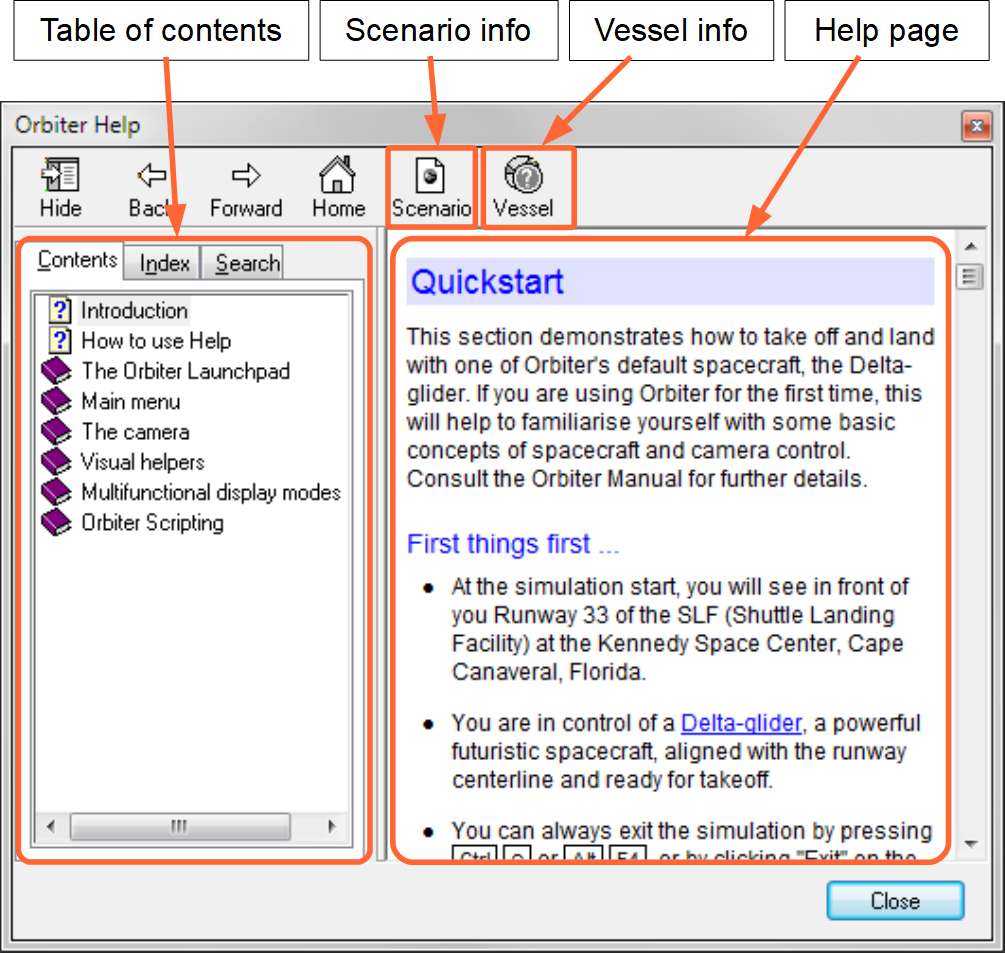
\includegraphics[width=0.5\textwidth]{help.png}}
\end{figure}

\noindent
The inline \textit{help} pages contain a subset of the topics covered in this manual, including

\begin{itemize}
\item Main menu and the dialogs accessible from it.
\item Camera control
\item Description of the MFD modes, including controls and display elements
\end{itemize}

\noindent
% TODO path (no more Orbitersdk\doc)
In addition, the inline help contains a chapter on Lua scripting and the Orbiter Lua extensions. Orbiter supports the Lua script language for a variety of tasks, including vessel control (via the Terminal MFD mode), autopilots, unsupervised vessel operation, mission design and tutorials. For a more detailed introduction to Lua scripting in Orbiter, see the Orbiter Lua Reference in Orbitersdk\textbackslash doc\textbackslash orbiter\_lua.chm.\\
Various dialogs in Orbiter have a Help button which provide context-sensitive help by jumping to the appropriate page in the inline help system.\\
Some vessel classes, as well as specific scenarios, come with their own sections for the inline help system. You can call these up with the Scenario and Vessel buttons at the top of the help window.\\
Add-on developers are encouraged to provide inline help pages for their vessels and custom scenarios to help users familiarise themselves with specific controls, properties and functions.


\subsection{Custom functions}
\label{ssec:menu_cust_func}
Plug-in modules (either included in the basic orbiter distribution or downloadable as 3$^{rd}$ party contributions from the Orbiter add-on repositories) may provide a user interface using a dialog or window that can be opened inside an Orbiter session. The \textit{Custom functions} dialog lists all active modules that allow opening an interface dialog box. It can be opened with the main menu \textit{function} button (shortcut: \Ctrl\keystroke{F4}).

\begin{figure}[H]
	\centering
	\subfigure{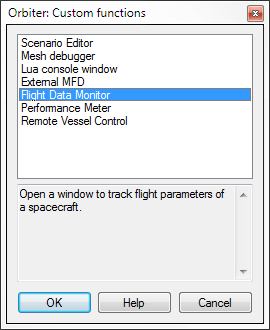
\includegraphics[width=0.35\textwidth]{custom_functions.png}}
\end{figure}

\noindent
Clicking on an entry shows a short description of the plug-in below the list. Double-clicking or the OK button opens the corresponding dialog.\\
A module must be \textit{activated} before it will be shown in the Custom functions dialog. See section \ref{ssec:launchpad_modules} on how to activate modules. Not all active modules may create an entry in the list. Some don't require user interaction and take effect as soon as they are activated.\\
See section \ref{sec:extra} for a description of some of the plug-in modules included in the Orbiter installation.


\end{document}
